% Gerado por scripts/gerar-figuras-monografia.py; não editar.
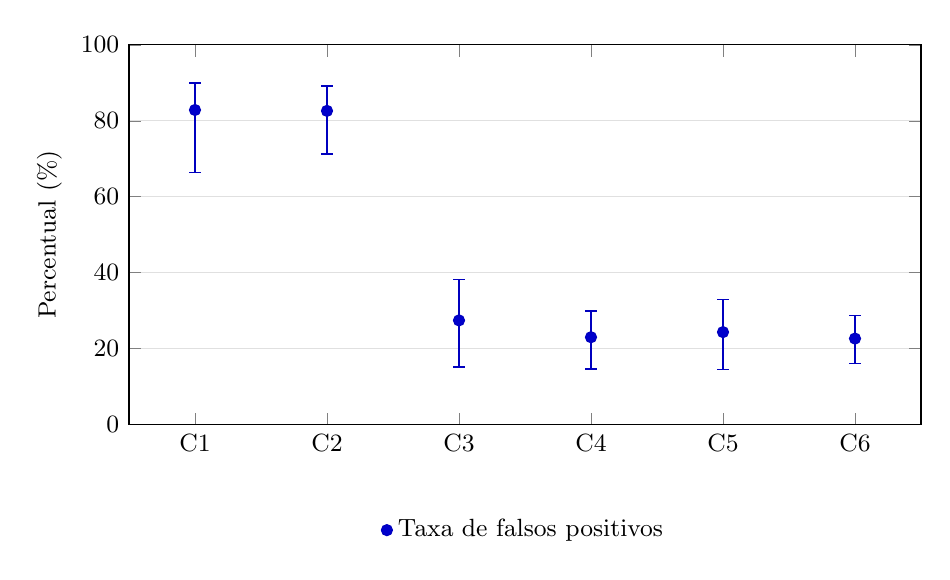
\begin{tikzpicture}
\begin{axis}[
width=0.96\textwidth,height=6.4cm,
tick label style={font=\small},label style={font=\small},
legend style={font=\small,at={(0.5,-0.22)},anchor=north,legend columns=3,draw=none,/tikz/every even column/.append style={column sep=8pt}},
ymajorgrids=true,grid style={black!12},
xmin=0.5,xmax=6.5,ymin=0,ymax=100,ylabel={Percentual (\%)},xtick={1,2,3,4,5,6},xticklabels={C1,C2,C3,C4,C5,C6}
]
\addplot+[only marks,mark=*,color=blue!75!black,error bars/.cd,y dir=both,y explicit] coordinates {(1.00000000,82.84883721) += (0,7.12111017) -= (0,16.50579514) (2.00000000,82.61538462) += (0,6.56855281) -= (0,11.35934597) (3.00000000,27.39170970) += (0,10.66985051) -= (0,12.26969440) (4.00000000,22.95877696) += (0,6.90046124) -= (0,8.38670716) (5.00000000,24.30522088) += (0,8.54667080) -= (0,9.79414146) (6.00000000,22.60480747) += (0,6.00662408) -= (0,6.66773359)};
\addlegendentry{Taxa de falsos positivos}
\end{axis}
\end{tikzpicture}
